\documentclass{article}
\usepackage{CJK}
\usepackage{graphicx}
\usepackage{listings}
\usepackage{mathtools}
\title{Project 1: Submit 1}
\author{Li Yin, Xiao Ao, Yang Qifan}
\date{November 2016}
\begin{document}

\maketitle
\begin{CJK}{UTF8}{gbsn}  

本次实验,我们对论文中提出的暴力法、Pwise、Uwise和Uwise+分别实现,并在给定的12个数据集以及NBA真实数据集上实验比较了不同算法的特点与优劣;接下来,我们将首先针对本次实验中出现的问题,交流优化和改进意见。

\section{算法描述}

\subsection{构建DSG}
DSG将多维点的集合按层存储,首层为skyline,第二层为次skyline,依次类推;在DSG中,点的parent为所有可以Dominate该点的集合,点的children为所有被该点Dominate的点集合。\\
程序实现:输入多维点的集合和层数k,输出一个k层的DSG。\\
$DirectedSkylineGraph$类实现了从一个Dataset和k构建DSG的静态方法。\\
\textbf{构建DSG}\\
首先将点集合按照第一维升序排序。对每一个点,分三种情况考虑:1.如果它不能被目前DSG的首层Dominate,那么它加入首层;2.如果它被最后一层Dominate并且DSG未达到k层,那么使用它来创建新的最后一层加入DSG中,如果此时的DSG已经达到k层,那么直接丢弃这个点;3.如果以上条件均不满足,则说明存在层i和其前一层i-1,层i不可以Dominate该点而层i-i可以,将点加入层i。\\
\textbf{构建Dominate关系}\\
目前所有点的parent和children关系比较简单,在如上描述构建好的DSG中,对每一层的每个点,遍历其上层所有的节点,如果它被上层节点压制了,则相互添加Dominate关系。\\
\textbf{点的Index}\\
对于最终保留在DSG中的点,按照第二维降序排列并赋予Index。
\subsection{Baseline与预处理}
Baseline使用枚举法求解G-Skyline groups。将DSG中的点所有集合长度为k的组合枚举出来后,过滤出不被其他组Dominate的组。\\
可以使用作者提出的预处理方法过滤点集合:如果某一点,其parent长度为k-1,则该点与其parent的集合为一个有效解;如果parent的长度大于k-1,则可不考虑该点;其余的点继续求解。预处理对baseline和后续算法均有效。

\subsection{Point-Wise}
在枚举树法进行G-Skyline groups的求解过程中,会产生庞大的时间与空间开销,于是论文中提出基于扩增点的方法进行树构建以及动态剪枝,最大程度地去掉冗余的部分,提高算法的效率,节省了计算过程的时间和空间。初始化树的第零层有一个根节点为空,tail set是预处理后得到的Directed skyline graph前k层的所有数据,然后从tail set中选取合适的点加入group中,第一层是加入1个点后所有满足条件的groups集合,第二层继续增加一个合适点,第3层,第4层以此类推,层数对应当层groups列表中每个group的元素个数。其中的剪枝优化主要有以下两个方面:\\
\textbf{子树修剪}
应用超集单调性这一性质,如果一个包含i个元素的集合$G_{i}$不是G-Skyline group,即使从其tail set中新增加一个点,组成的新的包含i+1个元素的集合$G_{i+1}$也不可能是G-Skyline group。所以在算法中,每从一个tail set中添加完一个合适的元素到原group得到的新group都要进行G-Skyline的判定,若新生成的group不是G-Skyline group,直接删除该节点,相当于直接去掉了一个以该节点为根节点的子树。\\
\textbf{Tail Set修剪}
根据文中引理G-Skyline group里面的点不能被除此group里面的元素以外的点所控制,即G-skyline group里每个元素只能是无父节点,或所有父节点在此group内。但这一步骤并不充分,若成功组成新group之后,得再次验证确保准确性。还有一个就是新加入的点必须保证在Directed Skyline Graph的前i+1层,若加入了大于等于i+2层以上的点,那么该点会被Gi以外的点所控制,不满足G-Skyline group定义。\\
其实,实现这个算法之后总结起来就是,每新加入的一个点首先是得在$G_{i}$的上一个加入的点对应的Directed Skyline Graph同一层找skyline点(即该层下标较大点),若已没有skyline点则向下一层i+1层寻找被$G_{i}$中元素控制的孩子即可。然后再循环建树的下一层,直到建完第k层截止,便可得到所有的满足条件的G-Skyline groups。\\
本算法按照论文中的伪码实现的,在实现过程中丰富了其中的细节,助教可查看源码,它实现了自GSkylineService接口。同时也在项目中定义了树节点PDataNode,方便计算。

\subsection{Group-Wise}
PWise算法以点为单位扩充叶节点,但是由于G-Skyline group中的一个点不能被其他group中的点dominate,所以也就是说某个节点的unit group(点及它的父亲节点)一定也在同一个group中;所以得到UWise算法,即以unit group为单位扩充叶节点。\\
为了提高效率,有两个剪枝的过程:Superset pruning和Tailset pruning。

\subsubsection{Superset pruning}
\textbf{去掉点个数超过k的candidate group,不再计算它的子树}
\begin{lstlisting}[language=C]
HashSet<DataPoint> union=get_union_unit_group(candidate);
if(union.size()==k){//get one result
    result.add(union);
    continue;
}else if(union.size()>k){//superset pruning
    continue;
}
\end{lstlisting}

\subsubsection{Tailset pruning}
\textbf{当前unit groups中的点的子节点,不再加入tailset}
\begin{lstlisting}[language=C]
private List<DataPoint> get_tail_Set(
    Set<DataPoint> set, List<DataPoint> points){

    List<DataPoint> tailSet=new ArrayList<>();
    HashSet<DataPoint> children=new HashSet<>();
    int maxIdx=-1;
    for (DataPoint p:set){
        int idx=points.indexOf(p);
        if(idx>maxIdx){
            maxIdx=idx;
        }
        //find all children points
        children.addAll(p.children);
    }
    for (int i=maxIdx+1;i<points.size();i++){
        if (!(children.contains(points.get(i)))){
            //remove it from tailset if it is in childrenset
            tailSet.add(points.get(i));
        }
    }
    return tailSet;
}
\end{lstlisting}

\subsection{UWise+}
UWise+在UWise基础上增加两个新的剪枝方法:Unit Group Reordering和Subset pruning。

\subsubsection{Unit Group Reordering}
因为Superset pruning对削减candidate group很有效,所以希望重新排列unit group来增强Superset pruning的效果,即先处理大的candidate group;所以按照点的检索倒序排列,即把高层的skyline layer的点排在前面。\\
此时我们还需要修改tailset,因为原来的子节点在重新排序后变成了父节点。\\

\subsubsection{Subset pruning}

如果一个candidate group $G_{i}$加上所有的tailset元素,即得到它子树中最深的子节点$G_{i}^{last}$,$G_{i}^{last}$的元素个数都不能达到k,则剪掉$G_{i}$,不去计算它的子树。
\begin{lstlisting}[language=C]
int gLast=get_last_deepest_candidate_group(p,points);
if(gLast<k){
    continue;
    }else if (gLast==k){
    Set<DataPoint> candidate
        =new HashSet<>(points.subList(0,points.indexOf(p)+1));
    result.add(candidate);
    continue;
}
\end{lstlisting}

\section{实验与评估}
\subsection{数据集}
本小组使用课程提供的anti,corr和inde三种类型的数据集,每类有2,4,6,8四种维度版本,共计12个数据集,并在论文提到的NBA数据网站下载球员数据,构建了1189条NBA球员的5维数据集。\\
所有实验使用的数据集位于项目目录的dataset文件夹内。构建数据集的脚本为nba/nba.py。其中需要提到的是,数据集中球员有某维度数据缺失,在本次实验中,我们拟合了缺失的数据。
\subsection{构建与使用方式}
构建:使用ant脚本,构建gskyline.jar包。\\
\begin{lstlisting}[language=C]
$ ant compile
\end{lstlisting}
运行示例:
\begin{lstlisting}[language=C]
java -Xms7G -Xmx8G -jar gskyline.jar all 4 datasets/*
java -jar gskyline.jar uwise+ 10 datasets/nba_5.txt
\end{lstlisting}
使用Java虚拟机参数配置可用的运行内存,较大的内存可以减少GC对算法的影响。\\
命令行参数分别为:\\
\begin{enumerate}
	\item method: 测试的算法名称,baseline,pwise,uwise或uwise+,all将对所有算法批量测试。
	\item k: 一个大于1的正整数,gskyline每组点的个数。
	\item files: 一个或是多个需要测试的数据文件。
\end{enumerate}
\subsection{实验运行环境}
OS: Ubuntu 14.04 x64\\
CPU: Intel Core 3317U @1.7Ghz\\
RAM: 2×4G DDR3 @1600Mhz\\
JDK: 1.8.0 60
\subsection{建立DSG与预处理}
DSG是后续所有算法运行依赖的数据结构,首先评估在不同数据集,不同K取值情况下,DSG构建所需的时间与DSG层数。\\

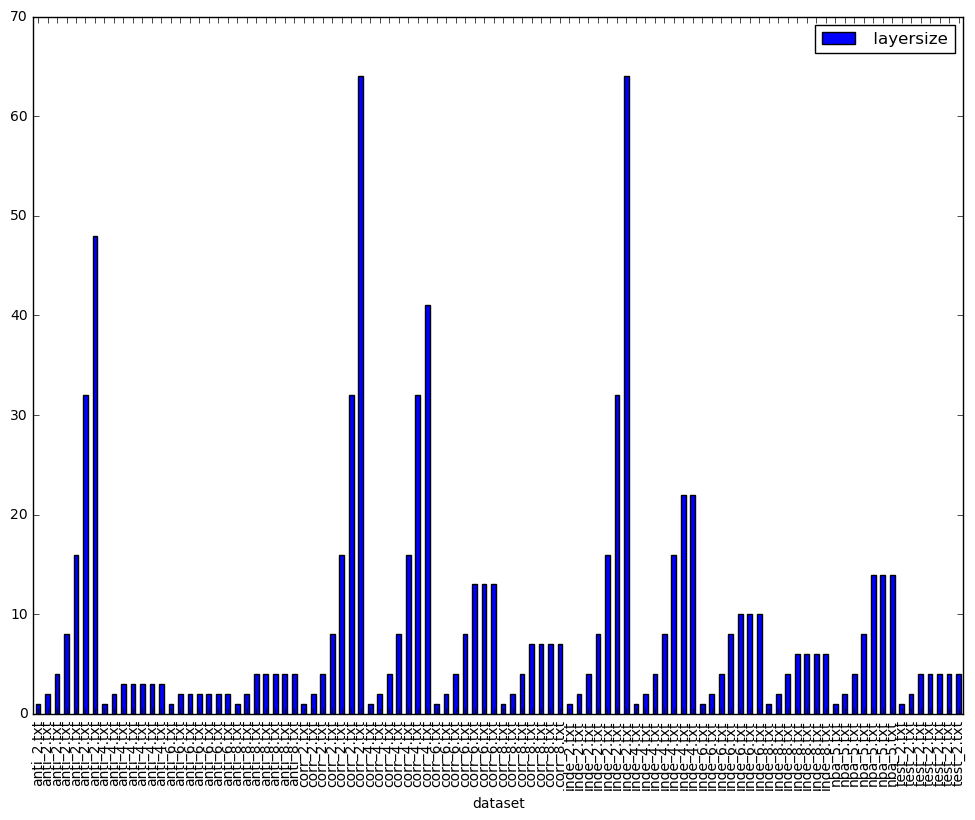
\includegraphics[scale=0.4]{pics/k_layer_size.png}\\
DSG层数与不同数据集、不同K取值的关系\\
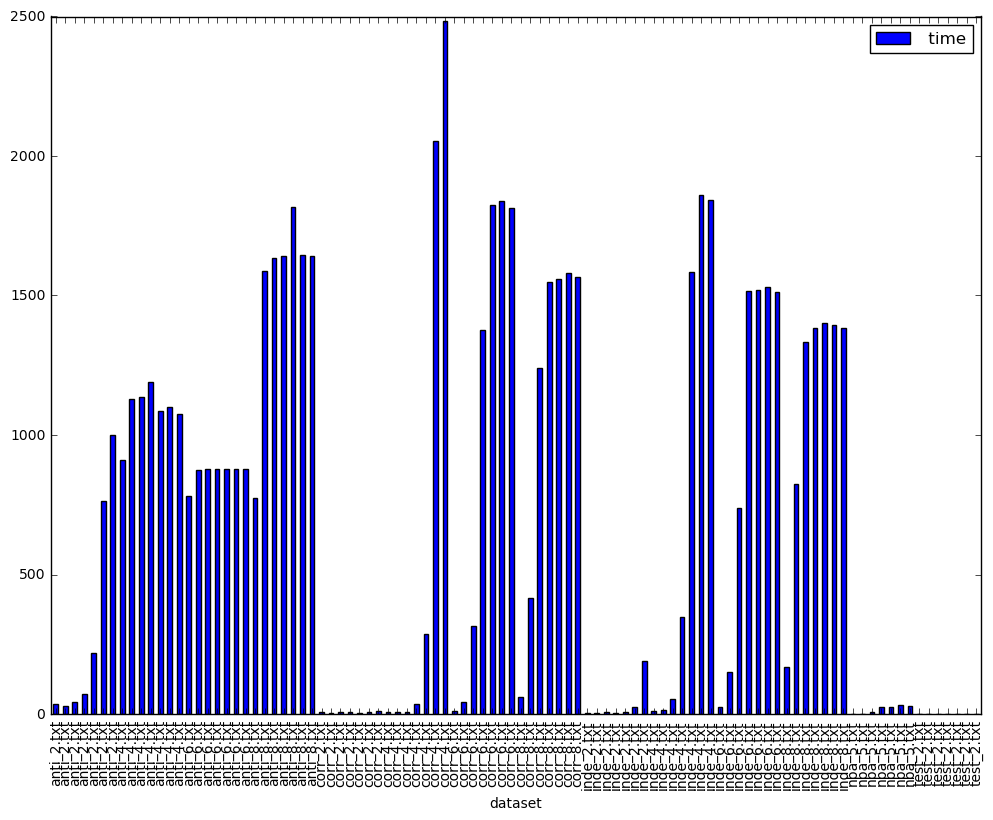
\includegraphics[scale=0.4]{pics/k_layer_time.png}
\\DSG构建时间与不同数据集、不同K取值的关系\\
从上两张图中我们可以看出,某些低纬度数据集的层数随着k值的不断加大呈现指数上升,如anti 2。还有些数据集随着k值的上升,其层数几乎不再上涨,这是因为其维度过高后,大多数节点直接很难确定胜负关系,如anti 4。\\
DSG构建的时间与DSG的层数呈现正相关。\\
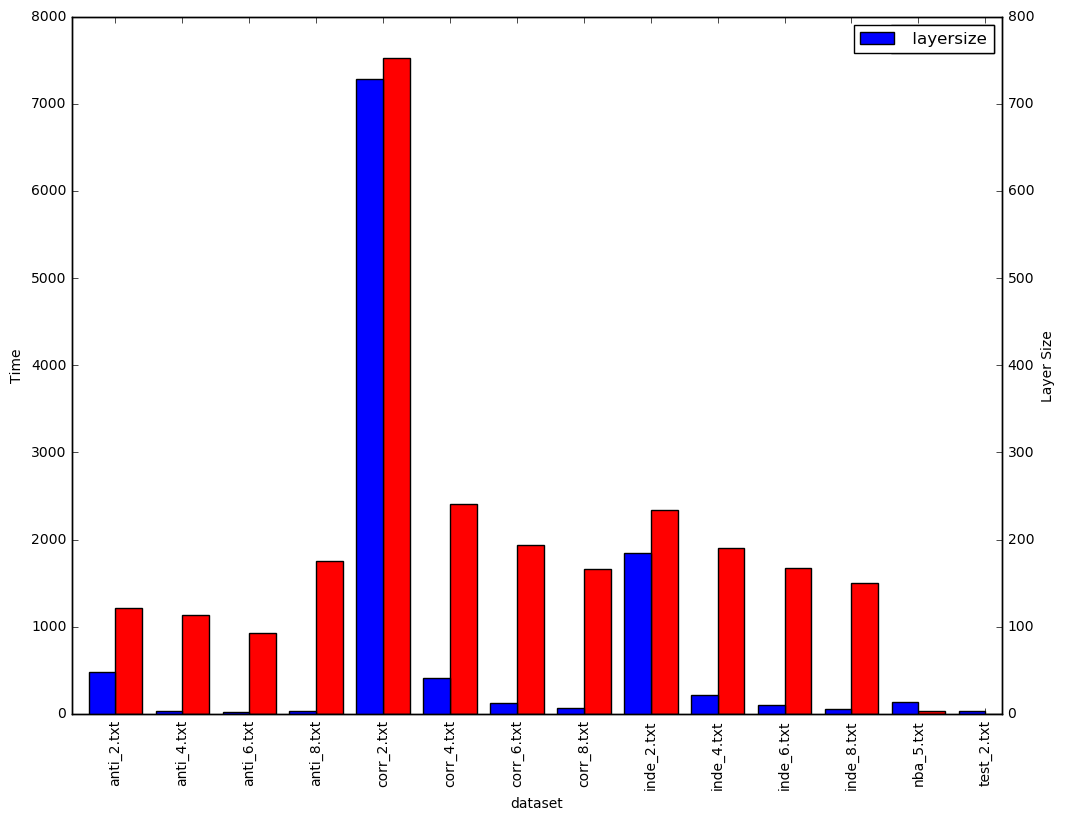
\includegraphics[scale=0.4]{pics/max_layer_building_time.png}
\\
全图构建时间(K足够大)与数据集的关系\\
由于DSG的构建与K相关,通过论文定理可知,组大小为K的GSkyline组的点只可能出现在前K层内,因此一般构建DSG中我们只构建前K层。如果K足够大,那么可以将所有点纳入DSG中。通过观察上图全图DSG的构建时间、构建层数与数据集的关系,可以观察到大多数10000点的DSG构建时间为秒级别,层数一般小于1000。图中corr 2的层数和构建时间超长,是我们接下来进行性能优化的一个研究点。\\
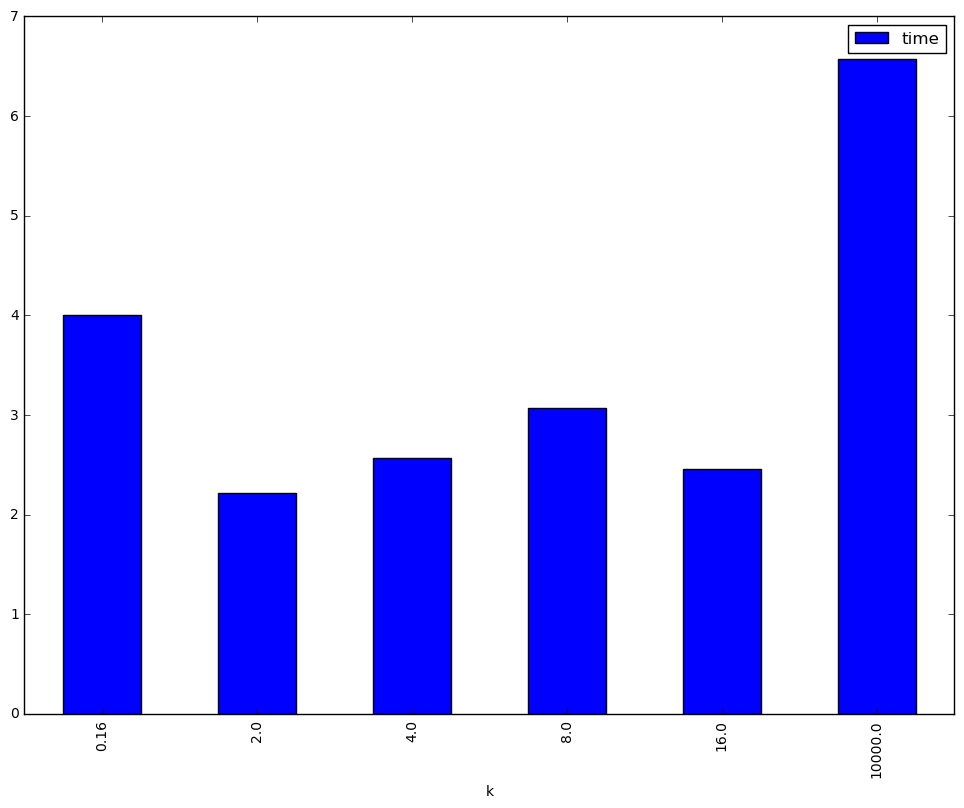
\includegraphics[scale=0.4]{pics/prefilter.png}\\
预处理时间与K值的关系\\
对点按照论文第五章进行预处理,可以通过点父亲节点的信息对点进行快速分别是否可能出现在group中,从上图可以看出,预处理的耗时很少,并且和K的大小没有直接的关系。\\
\subsection{计算G-Skyline Group}

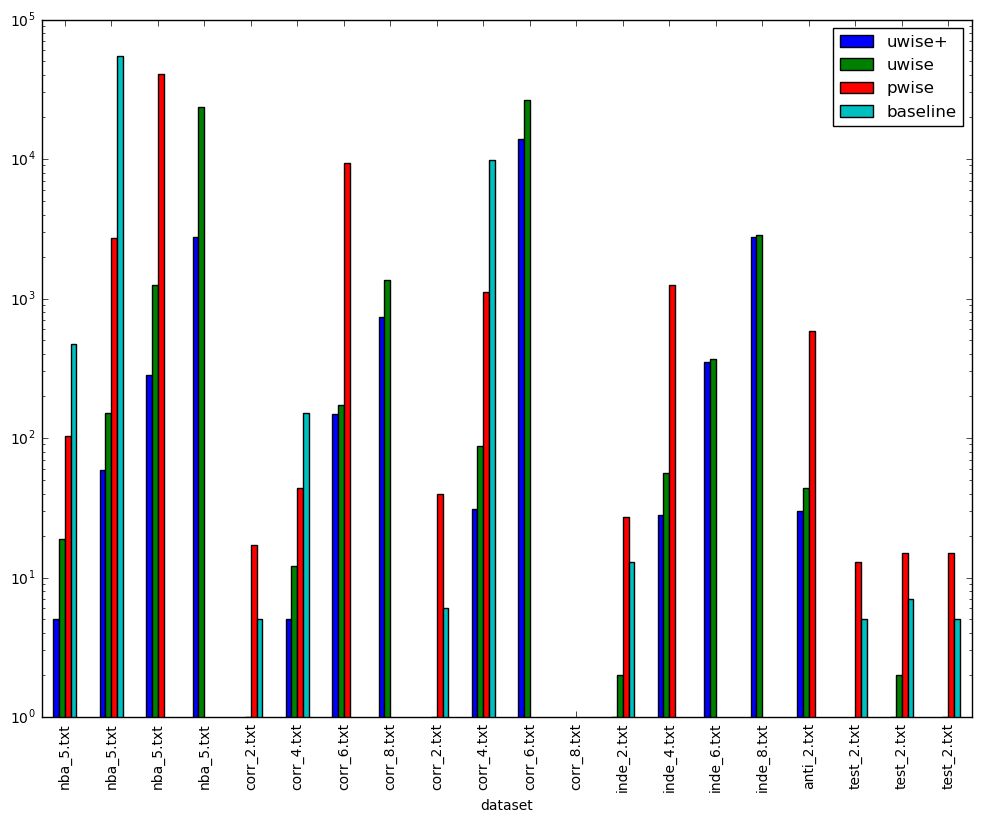
\includegraphics[scale=0.4]{pics/eval_4_algo_on_multi_dataset.png}
\\多个算法在不同数据集、不同K上的耗时\\
我们对实现的Baseline(暴力枚举)、Pwise、Uwise和Uwise+,在不同数据集和K取2-4的运行时间做了对比,此处使用的耗时不记录DSG的构建时间,但包括prefilter时间。\\
图中时间轴为Log增长。图表中有些数据为空,比如Baseline在图中多处缺失是因为耗时过长。\\
首先查看NBA数据集的结果。我们发现NBA数据集上算法耗时$uwise+ < uwise < pwise < baseline$。并且随着K的增大,每种算法的耗时都呈现指数级别增长。在k=4时,uwise+与uwise已经需要花费秒级别的耗时,而pwise和baseline已经不能在短时间内计算出结果。\\
在其他数据集和K的组合中,baseline可能在维度与K较小时候比pwise耗时更少,在一些数据集上uwise+虽然比uwise耗时少,但差距不是特别明显。\\
验证corr 8与anti 4数据集时,本Java实现需要耗费的内存大于6G,产生了严重的GC开销,最终难以计算出正确结果。优化本算法与程序实现的内存占用也是我们后续的一个优化方向。

\section{总结与下一步工作}
\begin{enumerate}
	\item 针对高内存占用,提出有效使用内存的算法或是程序实现,在我们的测试机器上防止因为内存占用而引发的高耗时。
	\item 在某些数据集上,例如corr 2的层数和DSG构建时间超长,提出更加高效构建DSG的算法。DSG是后续算法的依赖,并且DSG描述了多维数据间的复杂关系,可用于其他的问题和算法。
\end{enumerate}

\section{分工说明与感谢}
首先感谢组内同学,感谢助教查看与评估本实验报告。\\
肖翱完成了Point-Wise算法并完成了相应的文档。\\
李茵完成了Group-Wise和Group-Wise Plus算法并完成了相应的文档。\\
杨启凡完成了DSG构建和Baseline,完善了程序框架并评估了实验结果。\\
\end{CJK}
\end{document}
